\begin{center}
\large Experimento: \textbf{Amplificador de dois estágios com TJB}
\end{center}


\section{Introdução}

O presente relatório visa detalhar o experimento laboratorial realizado na disciplina laboratório de circuitos eletrônicos no dia 27 de agosto de 2019 sobre amplificador de dois estágios com transistores de junção bipolar (TJBs). 

Esse tipo de amplificador com múltiplos estágios são usados para conseguir m ganho maior e para promover um melhor controle das impedâncias de entrada e saída. Estes são os benefícios que o amplificador de múltiplos estágios tem em comparação ao de estágio único.

A prática objetiva a medição do ganho global e de cada estágio, bem como a impedância de entrada para um aplificador de dois estágios com TJB representado pelo esquemático da figura \ref{fig:1}. Para isso foram utilizados dois transistores BC 547B, com fatores de multiplicação de corrente de base o mais próximos possíveis ($Q_1: \beta = 263$ e $Q_2: \beta = 243$). 

Inicialmente realizou-se a análise DC, medindo o ponto de operaçãod e cada um dos transitores. Logo após, na análise AC foi injetada uma sinoide 1kHz de frequência e amplitude variável para que se observasse a saída (não saturada) e medisse o ganho global e de cada estágio. Por fim, foi medida a impedância de entrada do circuito com um sinal AC na entrada e com um resistor de valor conhecido para a criação de um divisor de tensão com a impedância de entrada.

\begin{figure}[H] 
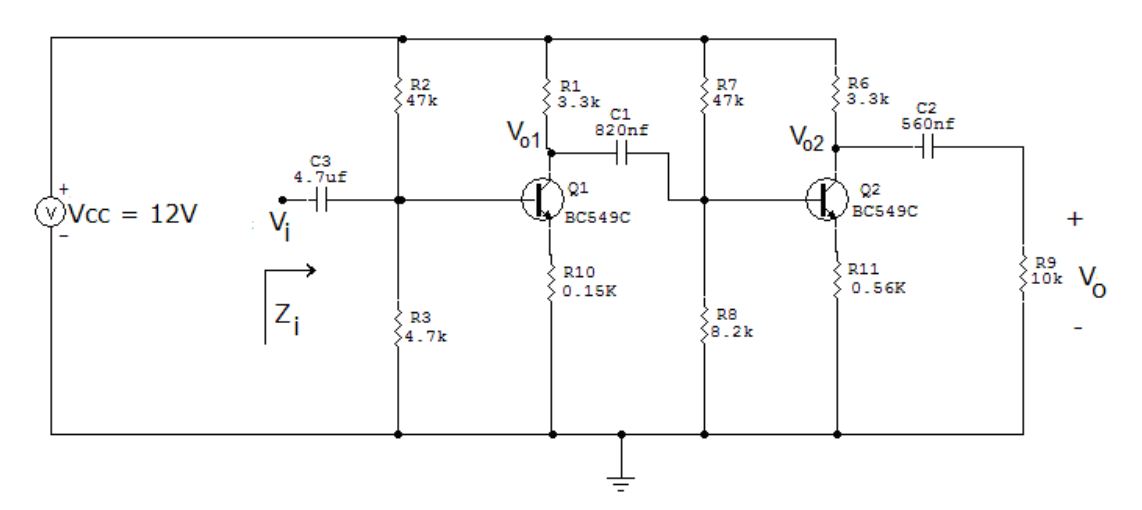
\includegraphics[scale=0.6]{imagens/ckt.png} 
\centering
\caption{Esquemático do amplificador de dois estágios.}
\label{fig:1} 
\end{figure} 

Com auxílio do multímetro digital da bancada foi medido o ponto de operação $V_{CE}$ e $I_C$ de cada estágio do circuito para cada transistor. Na análise AC a forma de onda de entrada foi gerada no gerador de sinais e as saídas foram obervadas no osciloscópio digital.


\section{Análise teórica}

\subsection{Análise DC}

Considera-se o circuito mostrado na figura \ref{fig:1} e a notação usada para cada componente. Dito isso, pode-se iniciar a primeira parte da análise do circuito, que é a análise DC, permitindo descobrir o ponto de operação de cada um dos transistores.

Devido à existência dos capacitores de acoplamento, o ponto de operação de cada um dos transistores poderá ser analisado individualmente, pois as tensões e correntes DC serão filtrados pelos capacitores.

Assim, considera-se que ambos os transistores estão em modo ativo para iniciar a análise.

Considera-se $I_{B1}$ e $I_{B2}$ desprezíveis em relação à corrente que passa no divisor de tensão. Assim as tensões nas bases são:

\begin{center}
    $V_{B1} = \frac{R_3}{R_3 + R_2}V_{CC}$  
    
    $V_{B2} = \frac{R_8}{R_8 + R_7}V_{CC}$
\end{center}

Considerando $V_{BE1}=V_{BE2}=V_{BE} \approx 0,7V$, a tensão em cada um dos emissores será:

\begin{center}
    $V_{E1} = V_{B1} - V_{BE} = \frac{R_3}{R_3 + R_2}V_{CC} - V_{BE}$
    
    $V_{E2} = V_{B2} - V_{BE} = \frac{R_8}{R_8 + R_7}V_{CC} - V_{BE}$
\end{center}

A corrente em cada emissor será:

\begin{center}
    $I_{E1} = \frac{V_{E1}}{R_{E2}} = \frac{1}{R_{10}} \left(\frac{R_3}{R_3 + R_2}V_{CC} - V_{BE} \right)$
    
    $I_{E2} = \frac{V_{E2}}{V_{E2}} = \frac{1}{R_{10}} \left(\frac{R_3}{R_3 + R_2}V_{CC} - V_{BE} \right)$
\end{center}

Considerando $\beta$ muito grande para ambos os transistores, tem-se que as correntes em cada um dos coletores são:

\begin{center}
    $I_{C1} = I_{E1} = 2,606mA$  
    
    $I_{C2} = I_{E2} = 1,933mA$  
\end{center}

Já as tensões entre coletor e emissor são dadas por:

\begin{center}
    $V_{CE1} = V_{C1} - V_{E1} = V_{CC} - I_{C1}(R_{1}-R_{10}) = 3,79V$  
    
    $V_{CE2} = V_{C2} - V_{E2} = V_{CC} - I_{C2}(R_{6}-R_{11}) = 4,54V$   
\end{center}

Com isso conclui-se a análise DC do circuito.

\subsection{Análise AC}

Com $V_T \approx 26mV$, tem-se que:
\begin{center}
    $g_{m1} = \frac{I_{C1}}{V_T} = 0.1 A/V$ 
    
    $g_{m2} = \frac{I_{C2}}{V_T} = 0.0743 A/V$ 
\end{center}

No que confere as resistências de saída de cada transistor, considera-as infinitas por desprezar o efeito Early ($V_A=\infty => r_o = \infty$). Já as resistências do modelo pi podem ser calculadas por:

\begin{center}
    $r_{\pi1} = \frac{\beta}{g_{m1}} = 2,63k\ohm$ 
    
    $r_{\pi2} = \frac{\beta}{g_{m2}} = 3,27k\ohm$ 
\end{center}

O circuito para pequenos sinais do primeiro estágio do amplificador é:

\begin{center}
\begin{tikzpicture}
    %shorts
    \draw (-0.5,0) node[left]{$v_i$} to[short,o-] (4,0) 
    (4,-2) to[short,-] (6,-2)
    (6,0) to[short, -o] (9.5,0) node[right]{$v_{o1}$} 
    (0.5,-2) to[short] (2,-2)
    %components (,) to[] (,){}
    (0.5,0) to[R,l=$R_2$,*-] (0.5,-2)
    (2,0) to[R,l=$R_3$,*-] (2,-2)
    (4,0) to[R,l=$r_{\pi 1}$, v=$v_{\pi1}$] (4,-2)
    (6,0) to[american controlled current source, l=$g_{m1}v_{\pi1}$, *-] (6,-2)
    (8.5,0) to[R,l=$R_1$,*-] (8.5,-2)
    (5,-2) to[R,l=$R_{10}$,*-] (5,-4)
    %ground
    (1.25,-2) node[ground]{} node[circ]{}
    (5,-4) node[ground]{} 
    (8.5,-2) node[ground]{}
    ;
\end{tikzpicture}
\end{center}

O circuito para pequenos sinais do segundo estágio do amplificador e com a carga é:

\begin{center}
\begin{tikzpicture}
    %shorts
    \draw (-0.5,0) node[left]{$v_{o1}$} to[short,o-] (4,0) 
    (4,-2) to[short,-] (6,-2)
    (6,0) to[short, -o] (11.5,0) node[right]{$v_{o}$} 
    (8.5,0.25)node[right]{$v_{o2}$} 
    (0.5,-2) to[short] (2,-2)
    (8.5,-2) to[short] (10,-2)
    %components (,) to[] (,){}
    (0.5,0) to[R,l=$R_7$,*-] (0.5,-2)
    (2,0) to[R,l=$R_8$,*-] (2,-2)
    (4,0) to[R,l=$r_{\pi 2}$, v=$v_{\pi2}$] (4,-2)
    (6,0) to[american controlled current source, l=$g_{m2}v_{\pi2}$, *-] (6,-2)
    (8.5,0) to[R,l=$R_6$,*-] (8.5,-2)
    (5,-2) to[R,l=$R_{11}$,*-] (5,-4)
    (10,0) to[R,l=$R_9$,*-] (10,-2)
    %ground
    (1.25,-2) node[ground]{} node[circ]{}
    (5,-4) node[ground]{} 
    (9.25,-2) node[ground]{} node[circ]{}
    ;
\end{tikzpicture}
\end{center}

O ganho do primeiro estágio vai depender da resistência de entrada do estágio seguinte, logo ele pode ser calculado como:

\begin{center}
     $a_{v1} = \frac{v_{o1}}{v_{i}} = \frac{-g_{m1}(R_{C1}//R_{in2})}{1+g_{m1}R_{E1}}$, com $R_{in2}=(r_{\pi2}+(\beta +1)R_{11})//R_7//R_8$
     
     $a_{v1} =  -13,8 V/V$
\end{center}

O ganho do segundo estágio pode ser calculado como:

\begin{center}
     $a_{v2} = \frac{v_{o2}}{v_{o1}} = \frac{-g_{m2}(R_{C2}//R_{L})}{1+g_{m2}R_{E2}} = \frac{-g_{m2}(R_6//R_9)}{1+g_{m2}R_{11}} = -4.326 V/V$
\end{center}

O ganho global será o produto entre os ganhos de ambos os estágios:

\begin{center}
     $a_{T} = a_{v1}a_{v2} = 59,7 V/V$
\end{center}

Com isso conclui-se a análise AC do circuito.

\subsection{Impedância de entrada}

A impedância de entrada pode ser dada como o paralelo entre a resistência de entrada para um amplificador de emissor comum degenerado ($r_{in} = r_{\pi1}+(\beta +1)R_{10}$ e $r_{\pi1}=\beta / g_{m1}$) com as duas resistências do divisor de tensão ($R_2$ e $R_3$) em paralelo, tendo que:

\begin{center}
     $z_{i} = \left(\frac{\beta}{g_{m1}}+(\beta +1)R_{10} \right)//R_2//R_3 = 3,87k\ohm$
\end{center}

\section{Metodologia}

Na prática a impedância de entrada foi calculada por meio da criação de um divisor de tensão na entrada com o primeiro estágio do circuito desconectado do segundo estágio e carga. Esse divisor consiste na impedância de entrada como icógnita e um resistor ($R_S$) de valor conhecido, escolhido arbitrariamente com a resistência de 4,7k\ohm.

De acordo com o circuito do ponto de vista AC da entrada inserida, fica-se:

\begin{center}
\begin{tikzpicture}
    %shorts
    \draw (0,3) to[sinusoidal voltage source, v=$v_1$] (0,0)
    (0,3) to[R=$R_S$] (3,3)
    to[R=$z_i$, v=$v_2$] (3,0)
    to[short] (0,0)
    ;
\end{tikzpicture}
\end{center}

Do divisor obtém-se a tensão $v_2$ e isola-se $z_i$ para obter a expressão:

\begin{center}
     $ z_{i} = R_S\frac{v_2}{v_1-v_2}$
\end{center}

Essa expressão foi utilizada juntamente com os valores medidos de tensão para calcular a impedância de entrada.

As demais medições foram feitas normalmente, matendo o cuidado de não saturar a saída para que ser possa obter os valores de tensão em cada um dos estágios para que possa calcular o ganho por meio dos valores medidos.

A tabela abaixo mostra os valores encontrados  em cada um das saídas para um sinal de entrada de 145mV de pico-a-pico e 1kHz:

\begin{table}[H]
\centering
\begin{tabular}{l|c|}
\hline
\multicolumn{1}{|l|}{\textbf{Tensão na saída do 1º estágio}} & 1,74V \\ \hline
\multicolumn{1}{|l|}{\textbf{Tensão na saída do 2º estágio}} & 7,44V \\ \hline
\end{tabular}
\caption{Valores medidos de tensão em cada estágio (os valores em questão são de pico-a-pico).}
\end{table}

As formas de onda correspondente aos sinais de tensão na saída de cada um dos estágios e para a medição do $z_i$ podem ser encontradas no anexo.

\section{Resultados e discussão}

Na atividade prática desenvolvida, além de fazemos medições do circuito amplificador de dois estágio foi preciso fazer uma análise matématica, para encontrar os parâmetros DC do sistema, quanto os parâmetros AC e verificar se as medições dos parâmetros calculados no circuito proposto foram aceitáveis.

Como foi considerado que ambos os transistores estão no modo ativo, logo $V_{BE1} \approx 0.7$ e $V_{BE2} \approx 0.7$, também foi considerado que o $\beta$ dos transistores é muito grande (da ordem $10^2$), logo podemos fazer uma aproximação de que $I_C \approx I_E$. Como se trata de transistores iguais as aproximações são exatamete iguais para ambos os transistores. Neste caso, foi possível encontrar, com ajuda do multímetro digital, um $\beta \approx 262 $ valores usuais do transistor BC547B utilizado, devido a falta de transistores BC549C. 

Para a análise DC foi calculado o ponto de operação ($V_{CE}$ e $I_{C}$), do mesmo modo da prática realizada anteriormente, foi medido de ambos resistores separadamente, ou seja, desconectados, devido que para componentes DC os capacitores se tornam um circuito aberto, como $C_1$ está entre ambos os transistores faz-se uma separação entre eles. Já para análise AC do circuito proposto foi montado o circuito equivalente de pequenos sinais do sistema e calculado seus ganhos parciais e o ganho global e a sua impedância de entrada, para isso foi preciso ultilizar um filtro disposto pelo o próprio oscilóscopio de forma a minimizar o efeito do ruído sobre o sistema para realizar as medições propostas.

Para efeitos de comparação foi montado uma tabela dos valores encontrados pela a análise matemática do circuito de dois estágios e os valores medidos em laboratório.



\begin{table}[H]
\centering
\begin{tabular}{l|c|c|}
\cline{2-3}
 & \textbf{\begin{tabular}[c]{@{}c@{}}Valores \\ Calculados\end{tabular}} & \textbf{\begin{tabular}[c]{@{}c@{}}Valores \\ Medidos\end{tabular}} \\ \hline
\multicolumn{1}{|l|}{\textbf{Ponto de Operação Q1}} & \begin{tabular}[c]{@{}c@{}}$V_{CE1}=3,79V$\\ $I_{C1}=2,606 mA$\end{tabular} & \begin{tabular}[c]{@{}c@{}}$V_{CE1}=3,93 V$\\ $I_{C1}=2,37 mA$\end{tabular} \\ \hline
\multicolumn{1}{|l|}{\textbf{Ponto de Operação Q2}} & \begin{tabular}[c]{@{}c@{}}$V_{CE2}=4,54 V$\\ $I_{C2}=1,933 mA$\end{tabular} & \begin{tabular}[c]{@{}c@{}}$V_{CE2}=4,59 V$\\ $I_{C2}=1,90 mA$\end{tabular} \\ \hline
\multicolumn{1}{|l|}{\textbf{Ganho do 1º Estágio ($v_{ol}$/$v_{i}$)}} & 13,8 V/V & 12 V/V \\ \hline
\multicolumn{1}{|l|}{\textbf{Ganho do 2º Estágio ($v_{ol}$/$v_{o2}$)}} & 4,326 V/V & 4,27 V/V \\ \hline
\multicolumn{1}{|l|}{\textbf{Ganho Total ($v_{o}$/$v_{i}$)}} & 59,7 V/V & 51,31 V/V \\ \hline
\multicolumn{1}{|l|}{\textbf{Impedância de Entrada}} & $3,87k\ohm$ & $3,497 k\ohm$ \\ \hline
\end{tabular}
\caption{Valores calculados e medidos para os parâmetros.}
\end{table}

Pela tabela podemos concluir que os valores teóricos foram bem aproximados com valores medidos, algums parâmetros divergiram um pouco mais, pois o erro acumulado para medições reais é muito alto e o sistema está muito propício a erros aleatórios.

Por fim, foi percebido que o pressuposto de que os transistores estavam em modo ativo é válido, pois as tensões de coletor-emissor são bem mais altas que 0,7 V, o que nos remete a polarização em modo ativo, isso era um problema que poderíamos enfrentar, pois o ganho do transistor BC547B é mais baixo que o do BC549C (que era o que deveria ter sido usado), mas no final temos os transistores em modo ativo.

Portanto, obtive-se uma boa amplificação, que já era esperado nos cálculos téoricos, pois temos um amplificador de dois estágios, como consideramos um transistor diferente do especificado, a análise  poderia nos causar problemas, mas no final tivemos a construção e o funcionamento do amplificador de dois estágios com sucesso.



\section{Conclusões}

Nesta prática foi estudado o amplificador TBJ de dois estágio, compreendendo como realizar sua montagem e fazendo as suas análise DC e AC do circuito proposto para encontrar seus parâmetros e comparar com valores calculados. Obtemos um ótimo resultado para o que nos foi proposto, assim concluimos que o amplificador possui um bom grau de amplificação. Além disso analisamos as dificuldades de montagem e cálculo dos parâmetros de circuitos de multiplos estágios, devido a complexidade imposta pelo sistema.    

\newpage

\section{Anexos}
Vide abaixo as formas de onda obtidas na prática:

\begin{figure}[H] 
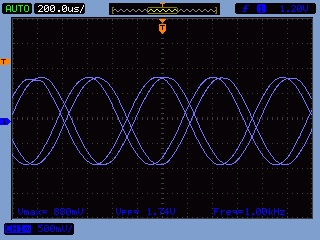
\includegraphics[scale=0.6]{imagens/174Vpp.jpg} 
\centering
\caption{Tensão na saída do primeiro estágio do amplificador.}
\label{fig:2} 
\end{figure} 

\begin{figure}[H] 
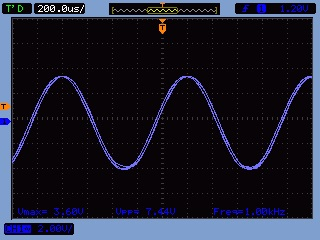
\includegraphics[scale=0.6]{imagens/744Vpp.jpg} 
\centering
\caption{Tensão na saída do segundo estágio do amplificador.}
\label{fig:3} 
\end{figure} 

\begin{figure}[H] 
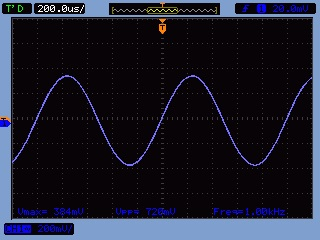
\includegraphics[scale=0.6]{imagens/720mVpp.jpg} 
\centering
\caption{Tensão $v_1$ para o cálculo de $z_i$.}
\label{fig:4} 
\end{figure} 

\begin{figure}[H] 
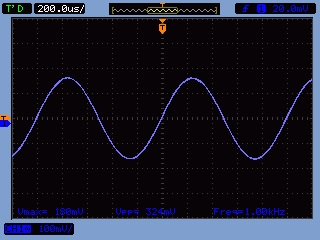
\includegraphics[scale=0.6]{imagens/324mVpp.jpg} 
\centering
\caption{Tensão $v_2$ para o cálculo de $z_i$}
\label{fig:5} 
\end{figure} 

Vide em anexo abaixo as folhas de cálculo utilizadas durante o experimento:

\begin{figure}[h!] 
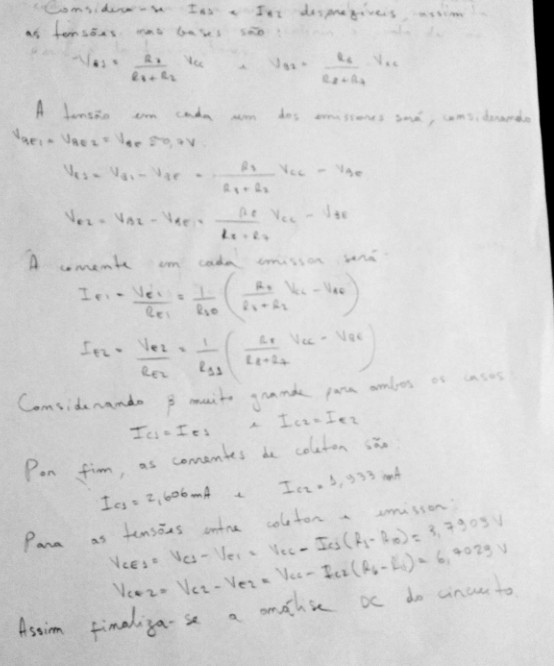
\includegraphics[scale=1]{imagens/calc1.png} 
\centering
\caption{Primeira folha de cálculos.}
\label{calc:1} 
\end{figure} 

\begin{figure}[h!] 
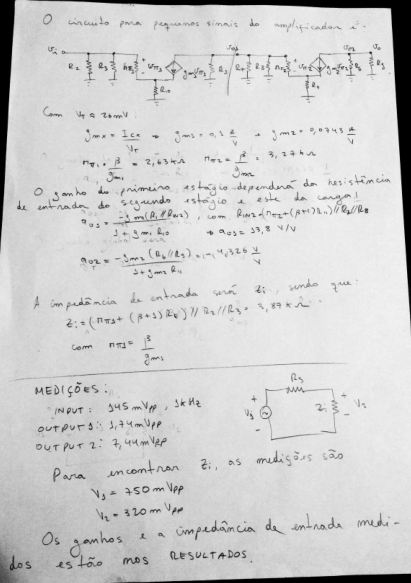
\includegraphics[scale=1]{imagens/calc2.png} 
\centering
\caption{Segunda folha de cálculos.}
\label{calc:2} 
\end{figure} 







     






